%\right \right \right \right \right \right \right \right \right \right \right \right \right \right \right \right \right \right \right \right \right \right \right \right \right \right \right \right \right \right \right \right \right \right \right \right \right \right \right \right \right \right \right \right \right \right \right \right \right 	~~~~~~~~```% This is "sig-alternate.tex" V2.0 May 2012
% This file should be compiled with V2.5 of "sig-alternate.cls" May 2012
%
% This example file demonstrates the use of the 'sig-alternate.cls'
% V2.5 LaTeX2e document class file. It is for those submitting
% articles to ACM Conference Proceedings WHO DO NOT WISH TO
% STRICTLY ADHERE TO THE SIGS (PUBS-BOARD-ENDORSED) STYLE.
% The 'sig-alternate.cls' file will produce a similar-looking,
% albeit, 'tighter' paper resulting in, invariably, fewer pages.
%
% ----------------------------------------------------------------------------------------------------------------
% This .tex file (and associated .cls V2.5) produces:
%       1) The Permission Statement
%       2) The Conference (location) Info information
%       3) The Copyright Line with ACM data
%       4) NO page numbers
%
% as against the acm_proc_article-sp.cls file which
% DOES NOT produce 1) thru' 3) above.
%
% Using 'sig-alternate.cls' you have control, however, from within
% the source .tex file, over both the CopyrightYear
% (defaulted to 200X) and the ACM Copyright Data
% (defaulted to X-XXXXX-XX-X/XX/XX).
% e.g.
% \CopyrightYear{2007} will cause 2007 to appear in the copyright line.
% \crdata{0-12345-67-8/90/12} will cause 0-12345-67-8/90/12 to appear in the copyright line.
%
% ---------------------------------------------------------------------------------------------------------------
% This .tex source is an example which *does* use
% the .bib file (from which the .bbl file % is produced).
% REMEMBER HOWEVER: After having produced the .bbl file,
% and prior to final submission, you *NEED* to 'insert'
% your .bbl file into your source .tex file so as to provide
% ONE 'self-contained' source file.
%
% ================= IF YOU HAVE QUESTIONS =======================
% Questions regarding the SIGS styles, SIGS policies and
% procedures, Conferences etc. should be sent to
% Adrienne Griscti (griscti@acm.org)
%
% Technical questions _only_ to
% Gerald Murray (murray@hq.acm.org)
% ===============================================================
%
% For tracking purposes - this is V2.0 - May 2012

\documentclass{sig-alternate}
\usepackage[normalem]{ulem}
\usepackage{algpseudocode}
\usepackage{algorithm}
\usepackage{amsmath}
%\usepackage{url}
\usepackage{graphicx}
\usepackage{subfigure}

\usepackage{footnote}
\makesavenoteenv{tabular}
\makesavenoteenv{table}

\algrenewcommand{\algorithmicrequire}{\textbf{Input:}}
\algrenewcommand{\algorithmicensure}{\textbf{Output:}}
\renewcommand{\algorithmicforall}{\textbf{for each}}

\begin{document}
%
% --- Author Metadata here ---
\conferenceinfo{WOODSTOCK}{'97 El Paso, Texas USA}
%\CopyrightYear{2007} % Allows default copyright year (20XX) to be over-ridden - IF NEED BE.
%\crdata{0-12345-67-8/90/01}  % Allows default copyright data (0-89791-88-6/97/05) to be over-ridden - IF NEED BE.
% --- End of Author Metadata ---

\title{Error Locating Driven Array\titlenote{This work was supported by the National Natural Science Foundation of China (No. 61272079), the Research Fund for the Doctoral Program of Higher Education of China (No.20130091110032), the Science Fund for Creative Research Groups of the National Natural Science Foundation of China(No. 61321491), and the Major Program of National Natural Science Foundation of China (No. 91318301)}
}
%
% You need the command \numberofauthors to handle the 'placement
% and alignment' of the authors beneath the title.
%
% For aesthetic reasons, we recommend 'three authors at a time'
% i.e. three 'name/affiliation blocks' be placed beneath the title.
%
% NOTE: You are NOT restricted in how many 'rows' of
% "name/affiliations" may appear. We just ask that you restrict
% the number of 'columns' to three.
%
% Because of the available 'opening page real-estate'
% we ask you to refrain from putting more than six authors
% (two rows with three columns) beneath the article title.
% More than six makes the first-page appear very cluttered indeed.
%
% Use the \alignauthor commands to handle the names
% and affiliations for an 'aesthetic maximum' of six authors.
% Add names, affiliations, addresses for
% the seventh etc. author(s) as the argument for the
% \additionalauthors command.
% These 'additional authors' will be output/set for you
% without further effort on your part as the last section in
% the body of your article BEFORE References or any Appendices.

\numberofauthors{3} %  in this sample file, there are a *total*
% of EIGHT authors. SIX appear on the 'first-page' (for formatting
% reasons) and the remaining two appear in the \additionalauthors section.
%
\author{
% You can go ahead and credit any number of authors here,
% e.g. one 'row of three' or two rows (consisting of one row of three
% and a second row of one, two or three).
%
% The command \alignauthor (no curly braces needed) should
% precede each author name, affiliation/snail-mail address and
% e-mail address. Additionally, tag each line of
% affiliation/address with \affaddr, and tag the
% e-mail address with \email.
%
% 1st. author
\and
 Xintao Niu and Changhai Nie\\
       \affaddr{State Key Laboratory for Novel}\\
       \affaddr{ Software Technology}\\
       \affaddr{Nanjing University, China}\\
%       \affaddr{China, 210023}\\
       \email{niuxintao@gmail.com}\\
       \email{changhainie@nju.edu.cn}
  %     \email{changhainie@nju.edu.cn}
% 2nd. author
\alignauthor
Hareton Leung \\
       \affaddr{Department of computing}\\
       \affaddr{Hong Kong Polytechnic University}\\
       \affaddr{Kowloon, Hong Kong}\\
       \email{ cshleung@comp.polyu.edu.hk}
% 3rd. author'
%\alignauthor
%Jeff Lei\\
%       \affaddr{Department of Computer Science and Engineering }\\
%       \affaddr{The University of Texas at Arlington}\\
%       \affaddr{Arlington, Texas}\\
%       \email{ylei@cse.uta.edu }
% 3rd. author'
%\and
\alignauthor
JiaXi Xu\\
       \affaddr{School of Mathematics and Information Technology}\\
       \affaddr{Nanjing Xiaozhuang University}\\
       \affaddr{China, 211171}\\
       \email{xujiaxi@126.com}
}
% There's nothing stopping you putting the seventh, eighth, etc.
% author on the opening page (as the 'third row') but we ask,
% for aesthetic reasons that you place these 'additional authors'
% in the \additional authors block, viz.
% Just remember to make sure that the TOTAL number of authors
% is the number that will appear on the first page PLUS the
% number that will appear in the \additionalauthors section.
\maketitle
\begin{abstract}
Combinatorial testing(CT) seeks to handle potential faults caused by various interactions of factors that can influence the Software systems. When applying CT, it is a common practice to first generate a bunch of test cases to cover each possible interaction and then to locate the failure-inducing interaction if any failure is detected. Although this conventional procedure is simple and straightforward, we conjecture that it is not the ideal choice in practice. This is because 1) testers desires to isolate the root cause of failures before all the needed test cases are generated and executed 2) the early located failure-inducing interactions can guide the remaining test cases generation, such that many unnecessary and invalidate test cases can be avoided. For this, we propose a novel CT framework that allows for both generation and localization process to better share each other's information, as a result, both this two testing stages will be more effectively and efficiently when handling the testing tasks. We conducted a series of empirical studies on several open-source software, of which the result shows that our framework can locate the failure-inducing interactions more quickly than traditional approaches, while just needing less test cases.
%When the system under test(SUT) is suffered from interations faults such as option compliant, testers want to design. As . Efficenet test space is desired when . To handle this problem, the art of  is to design a t-way covering array, which can cover all the t-way , just using small size of test cases. In this paper, however, we conjecture that the covering array is somewhat reduntant with respect to fault locating. The main reason for the reduntance the we find is the framework it takes is not efficent, traditional works will first generate a covering array to detect if any failing is triggered by any test case, and then pick these failing test case to further locating. In CT, most locating teachinques is just to generate addtional test cases to isolate the MFS. We find two shortcoming for this framework 1: if we had first identify some MFS, we do not need to generate any test case to conatin them, further, any combination contain this MFS will not need to be covered, 2: if we do not genrate, the extra test cases will support some coverage is that when we first already covered. So for this two points, in this paper, we propose a new framework to make the generating process and isolating process more tightly so that the isolating process and generating process will better utilize each other. We have done some emprical studies on several open-source software and found that our new frame work can significantly reduce the test cases.
%Combinatorial testing(CT) is proven to be effective to reveal the potential failures caused by the interaction of the inputs or options of the System Under Test(SUT). A key problem in CT is to isolate the failure-inducing combinations of the related failure as it can facilitate the debugging efforts by reducing the scope of code that needs to be inspected. Many algorithms has been proposed to identify such combinations, however, most of these studies either just consider the condition of one fault or ignore masking effects among multiple faults which can bias their identified results. In this paper, we analysed how the masking effect of multiple faults affect on the isolation of failure-inducing combinations. We further give a strategy of selecting test cases to alleviate this impact, which works by pruning these test cases that may trigger masking effect and replacing them with no-masking-effect ones. The test case selecting process repeated until we get enough information to isolate the failure-inducing combinations. We conducted some empirical studies on several open-source software. The result of the studies shows that multiple faults as well as the masking effects do exist in real software and our approach can assist combinatorial-based failure-inducing identifying methods to get a better result when handling multiple faults in SUT.
\end{abstract}

% A category with the (minimum) three required fields
%\category{H.4}{Information Systems Applications}{Miscellaneous}
%A category including the fourth, optional field follows...
\category{D.2.5}{Software Engineering}{Testing and debugging}[Debugging aids,testing tools]

\terms{Reliability, Verification}

\keywords{Software Testing, Combinatorial Testing, Covering Array, Failure-inducing combinations} % NOT required for Proceedings

\section{Introduction}

Modern software is developed more sophisticatedly and intelligently than before. To test such software is challenging, as the candidate factors that can influence the system's behaviour, e.g., configuration options, system inputs, message events, are enormous. Even worse, the interactions between these factors can also crash the system, e.g., the compatibility problems. In consideration of the scale of the real industrial software, to test all the possible combination of all the factors (we call them the interaction space) is not feasible, and even it is possible, it is not recommended to test exhaustive interactions for most of them do not provide any useful information.

Many empirical studies shows that in real software systems, the effective interaction space, i.e., targeting fault defects, makes up only a small proportion of the overall interaction space. What's more, the number of factors involved in these effective interactions is relatively small, of which 4 to 6 is usually the upper bonds. With this observation, applying CT in practice is appealing, as it is proven to be effective to handle the interaction faults in the system.

A typical CT life-circle is listed as Figure \ref{ct-life}, in which there are four main testing stages. At the very beginning of the testing, engineers should extract the specific model of the software under test. In detail, they should identify the factors, such as user inputs, configure options, environment states and the like that could affect the system's behavior. Next, which values each factor can take should also be determined. Further efforts will be needed to figure out the constraints and dependencies between each factor and corresponding values to make the testing work valid. After the modeling stage, a bunch of test cases should be generated and executed to expose the potential faults in the system. In CT, one test case is a set of assignment of all the factors that we modeled before. Thus, when such a test case is executed, all the interactions contained in the test case are deemed to be checked. The main target of this stage is to design a relatively small size of test cases to get some specific coverage, for CT the most common coverage is to check all the possible interactions with the number of factors no more than a prior fixed integer, i.e., strength \emph{t}. The third testing stage in this circle is the fault localization, which is responsible for diagnosing the root cause of the failure we detected before. To characterize such root cause, i.e., failure-inducing interactions of corresponding factors and values is important for future bug fixing, as it will reduce the suspicious code scope that needed to inspect. The last testing stage of CT is evaluation. In this stage, testers will assess the quality of the previously conducted testing tasks, many metrics such as whether the failure-inducing interactions can reflect the failures detected, whether the generated test cases is adequate to expose all the behaviors of the system,  will be validated. And if the assessment result shows that the previous testing process does not fulfil the testing requirement, some testing stages should be made some improvement, and sometimes, may even need to be re-conducted.

Although this conventional CT framewbach2004pairwiseork is simple and straightforward, however in terms of the test cases generation and fault localization stages, we conjecture that the first-generation-then-localization is not the proper choice for most test engineers. This is because, first, it is not realistic for testers wait for all the needed test cases are generated before they can diagnosis and fix the failures that haven been detected \cite{yoo2013fault}; second, and the most important, utilizing the early determined failure-inducing interactions can guide the following test cases generations, such that many unnecessary and invalid test cases will be avoided. For this we get to the most key idea of this paper:

\emph{Generation and Localization process should be organised in a more tightly way.}

Based on the idea, we propose a new CT framework, which instead of dividing the generation and localization into two independent stages, it integrate this two stages into one. We call this new one the Generation-Localization stage, which allows for both generation and localization better share each other's testing information. To this aim, we remodel the generation and localization module to make them better adapt to this newly framework. In specific, our generation adopts the one-test-one-time strategy, i.e., generate and execute one test case in one iteration. Rather than generating the overall needed test cases in one time, this strategy is more flexible so that it allows for terminating at any time during generation, no matter whether the coverage is reached or not. With this strategy, we can let the generation stops at the point we detect some failures, and then after localization we can utilize the diagnosing result to change the coverage criteria, e.g., the interactions related to the failure-inducing interactions do not need to be checked any more. Then based on the new coverage criteria, the generation process goes on.

%For the fault localization, we augment this process with a test case . instead of independently generating extra test cases, we add a new process to let it can get a guide . we will also take use of the test cases generation before, this will shows in the extra test case. Fault localization will need more.

We conducted a series empirical studies on several open-source software to evaluate our newly framework. In short, we take two main comparisons, one is to compare our new framework with the traditional one, which first generate a complete set of test cases and then perform the fault localization. Another one is to compare with the Error locating array, which is a well-designed set of test cases that can be used directly detect and isolate the failure-inducing interactions. The results shows that in terms of test case generation and fault diagnosis, our approach can and significantly reduced the overall needed test cases and can more quickly isolate the root cause of the system under test.

The main contributions of this paper:

 \begin{enumerate}
 \item  We propose a newly CT framework which combine the test cases generation and fault localization more closely.
 \item  We augment the traditional CT test cases generation and fault localization process to make them adapt to the newly framework.
 \item  A series comparisons with traditional CT is conducted and the result of the empirical studies are discussed.
\end{enumerate}


The reset of the paper is organised as follows: Section 2 presents the preliminary background of some definitions of the CT.  Section 3 describes our newly framework and a simple case study is also given. Section 4 presents the empirical studies and the results are discussed. Section 5 shows the related works. Section 6 concludes the paper and propose some further works.


% Cohen[] studies the , and find 70 ~ 100 can be. []Shows that to get a some coverage, only a small subset of all the configuration is needed. To this aim,
%
%Typically, when applying CT in practice, there are four testing stages that should be cated as in figure. At the very early of the testing work, engineers should characterize which options and what inputs , i.e., to identify the factors and their possible values. This stage is labor-consuming, at least in the initial testing. The second stage is to generate a bunch of test cases to meet some criteria. In CT, the most common scenario is to cover all the iterations with the factors in the interactions no more than a prior fixed number -- t, in such way, the test suites of CT is also called the t-way covering array.  The third testing stage is to fault localization, i.e., to isolate the failure-inducing interactions which owes to those failures triggered in those test cases in these test cases. The final stage is to evaluate the quality of the test cases.
%
%This conventional CT framework is simple and straight forward, however, we conjecture, it is not he suiable choices and not the choices for most test engineers.  The first,   Second, and most importantly, is.
%
%For this, we.


\begin{figure}
 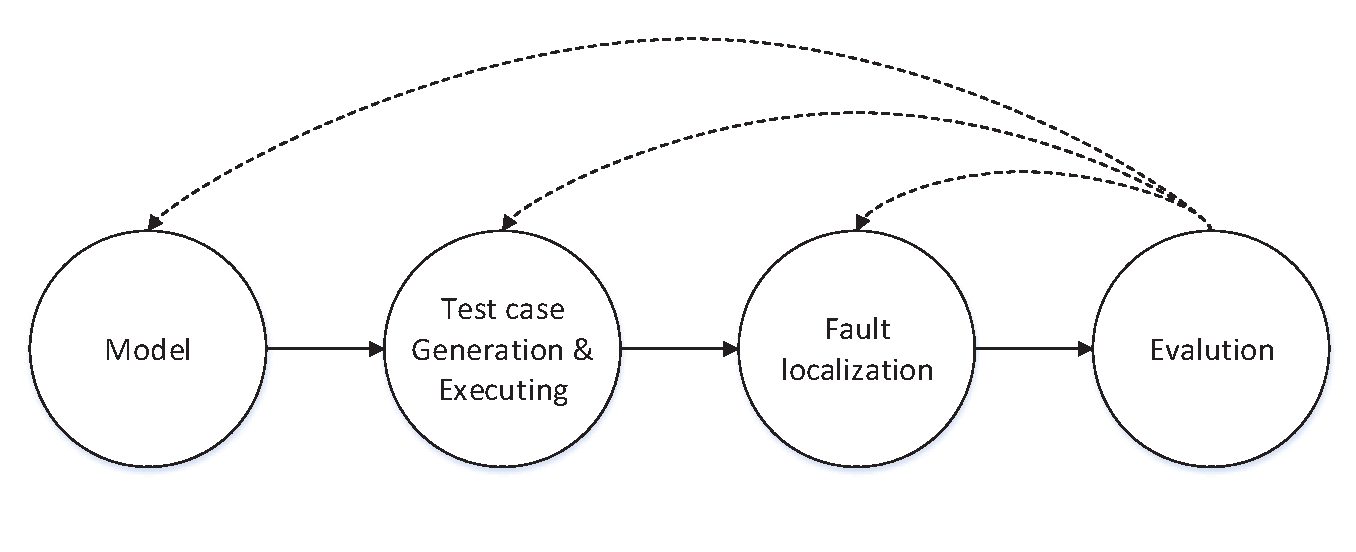
\includegraphics[width=3.4in]{CT_lifecircle.eps}
\caption{The life circle of CT}
\label{ct-life}
\end{figure}
%Software system are growing more and more complexity, the testing is needed. Nowadays, the bugs are not the single factor-bug, that is, it is . To detect and isolate such a is hard, for we could not easily know which interaction of from so many. The first, how to detect, the second, even if we have detected, .


%
%Combinatorial testing is a proposing testing technique to handle such problem. The testing object-- covering array is a well designed test suite, which can cover each possible interaction with just a small or reasonable size. When one or more test cases trigger some fault, it take the isolating.asdlajsdlas-d=
%
%In CT it is a pri-critira that the test suite must be , and then using to trigger. This framework is straight and simple, however, we conjecture in this paper that this would be more redundant inspect of fault debugging. Through a series experiment on empirical study, we observe that, there is two main : right . wrong .   This redundant can make the tester to test more unnecessary test cases, which is a wasting of computing resource.
%
%So in this paper, we propose a new and really intuial CT fault detecting and isolating framework (CTDI), which combine the more tightly. In detail our framework, handles two main . For we find . we make it as constraint, and feedback to the generating. The second, as we can generate many extra test cases, for these passing test cases, we use them as seed to let them in the generating process. The ended criteria is some coverage is reached.
%
%Our new CT is .
%
%We have imply , and find our approach can .



%
%With the increasing complexity and size of modern software, many factors, such as input parameters and configuration options, can influence the behaviour of the SUT. The unexpected faults caused by the interaction among these factors can make testing such software a big challenge if the interaction space is too large. One remedy for this problem is combinatorial testing, which systematically sample the interaction space and select a relatively small set of test cases that cover all the valid iterations with the number of factors involved in the interaction no more than a prior fixed integer, i.e., the \emph{strength} of the interaction.
%
%Once failures are detected, it is desired to isolate the failure-inducing combinations in these failing test cases. This task is important in CT as it can facilitate the debugging efforts by reducing the code scope that needed to inspected.

%\section{Motivating example}
%Combinatorial testing can effectively detect the failures caused by the interactions between various options or inputs of the SUT. Covering arrays, the test suite generated by this technique can cover each combination of the options at least once. We conjecture, however, although covering array can effectively, in practice, covering array was too much for detecting and locating the error in particular software.
%
%As an motivating example, we looked through the following scenarios for detecting and locating the errors in the SUT.
%
%Too much redundant fault test cases:
%
%
%Too much redundant right test cases:

\section{Background}
This section presents some definitions and propositions to give a formal model for the FCI problem.

%\subsection{Failure-inducing combinations in CT}

Assume that the SUT is influenced by \emph{n} parameters, and each parameter $p_{i}$ has $a_{i}$ discrete values from the finite set $V_{i}$, i.e., $a_{i}$ = $|V_{i}|$ ($i$ = 1,2,..n). Some of the definitions below are originally defined in .

\newdef{definition}{Definition}
\begin{definition}
A \emph{test case} of the SUT is an array of \emph{n} values, one for each parameter of the SUT, which is denoted as a \emph{n}-tuple ($v_{1}$, $v_{2}$,...,$v_{n}$), where $v_{1}\in V_{1}$, $v_{2} \in V_{2}$ ... $v_{n} \in V_{n}$.
\end{definition}

In practice, these parameters in the test case can represent many factors, such as input variables, run-time options, building options or various combination of them. We need to execute the SUT with these test cases to ensure the correctness of the behaviour of the software.

%\begin{definition}
We consider the fact that the abnormally executing test cases as a \emph{fault}. It can be a thrown exception, compilation error, assertion failure or constraint violation. When faults are triggered by some test cases, what is desired is to figure out the cause of these faults, and hence some subsets of this test case should be analysed.
%\end{definition}

%Figuring out the test case as well as the executing result is usually not enough to analyse the source of the bug, especially when there are too many parameters we need to care in this test case. In this circumstance, we need to study some subsets of this test case, so we need the following definition:

%Figuring out the execution outcomes of test cases must reveal the presence of faulty interactions among those considered. However, the location and magnitude of the fault is still far from clear, especially when there are too many parameters we need to care in this test case. Hence, we need to study some subsets of this test case, which can help isolate the cause of failures.

\begin{definition}
For the SUT, the \emph{n}-tuple (-,$v_{n_{1}}$,...,$v_{n_{k}}$,...)is called a \emph{k}-value \emph{combination} ($0 < k \leq n $) when some k parameters have fixed values and the others can take on their respective allowable values, represented as ``-".

In effect a test case itself is a k-value \emph{combination}, when k = n. Furthermore, if a test case contain a \emph{combination}, i.e., every fixed value in the combination is in this test case, we say this test case \emph{hits} the \emph{combination}.
%, which can be denoted as $k-value\  combination \in T$
\end{definition}

\begin{definition}
let $c_{l}$ be a \emph{l}-value combination, $c_{m}$ be an \emph{m}-value combination in SUT and $l < m$. If all the fixed parameter values in $c_{l}$ are also in $c_{m}$, then $c_{m}$ \emph{subsumes} $c_{l}$. In this case we can also say that $c_{l}$ is a \emph{sub-combination} of $c_{m}$ and $c_{m}$ is a \emph{parent-combination} of $c_{l}$, which can be denoted as $c_{l} \prec  c_{m}$.
\end{definition}

For example, in the motivation example section, the 2-value combination (-, 4, 4, -) is a sub-combination of the 3-value combination (-, 4, 4, 5), that is, (-,4,4,-) $\prec$ (-,4,4,5).

\begin{definition}
If all test cases contain a combination, say $c$, trigger a particular fault, say $F$, then we call this combination $c$ the \emph{faulty combination} for $F$. Additionally, if none sub-combination of $c$ is the \emph{faulty combination} for $F$, we then call the combination $c$ the \emph{minimal faulty combination} for $F$ (It is also called Minimal failure-causing schema(MFS) in ).

%Based on this, if a test case $t$ hit such a failure-inducing combination, say $c(F)$, it should trigger the fault $F$, for which the test case can be put as $t(F)$
\end{definition}

In fact, MFS and \emph{minimal faulty combinations} are identical to the failure-inducing combinations we discussed previously. Figuring it out can eliminate all details that are irrelevant for causing the failure and hence facilitate the debugging efforts.

\subsection{Detect the failure-inducing schemas}
When applying CT on software testing, the most important work is to determine whether the SUT is suffering from the interaction faults or not, i.e., to  detect the existence of the MFS. Rather than impractically executing exhaustive test cases, CT commonly design a relatively small size of test cases to cover all the schemas with the degree no more than a prior fixed number, $t$. Such a set of test cases is calling the \emph{covering array}.  If some test cases in the covering array failed after execution, then the interaction faults is regard to be detected.

Many studies in CT field focus on how to generate such a test suite with the aim that making the size of the test suite as small as possible. In general, most of these studies can be classified into three categories according to the construction way of the covering array:

1) One test case one time : This strategy repeats generating one test case as one row of the covering array and counting the covered schemas so far until no more schemas is needed to be covered.

%  generate a completed test case to cover

2) A overall set of test cases one time:  This strategy first generates a set of test cases with the size of the set fixed in prior. Then through some operation such as mutation of the some cells, increase or decrease the size of the set of test cases, regeneration some test cases to make the set of test cases to cover all the needed schemas with the size as small as possible \cite{cohen2003augmenting}.

3) Others :  This strategy differentiates from the previous two strategies at the point it does not first give completed test cases \cite{lei2008ipog}. It will first focus on assigning values to some  particular factors or parameters to cover the schemas that related to these factors, and then complement the remaining part to form completed test cases.

In this paper, we focus on the first one: One test case one time as it can allow for immediately getting a completed test case such that the testers can execute and diagnosis in the early stage. And we will see later, with respect to the fault defeating, this strategy is the most flexible and efficient one comparing with the other two strategies.

%To isolate the failure-inducing schemas and further bug fixing, the first step, is to detect them. To efficiently isolate the failure-inducing schemas, and to . Such a testing object, is covering array, which ,. Formally,
%
%\begin{definition}
%Covering array.
%\end{definition}

%Such a covering can , how to generate such a covering lying two facts.
%There are three different kinds of generation
%
%Overall test
%
%one test one time
%
%other special testing object.

%In order to fulfil the testing target, we choose the second object, one test one time, as we can .

\subsection{Isolate the failure-inducing schemas}
To detect the existence of MFS in the SUT is still far from figuring out the root cause of the failure. As we do not know exactly which one or some schemas in the failed test cases should be responsible for the failure. In fact, for a failing test case, there can be at most $2^{k} - 1$ possible schemas can be the MFS. Hence, further fault diagnosis is desired, i.e., more test cases should be generated to isolate the MFS.

A typical MFS isolating process is as Table \ref{ofot-identify}. This example assumes the SUT has 3 parameters, each can take 2 values. And assume the test case (1, 1, 1) failed. Then in Table \ref{ofot-identify}, as test case \emph{t} failed, and OFOT mutated one factor of the \emph{t} one time to generate new test cases: $t_{1}$ -- $t_{3}$, It found the the $t_{1}$ passed, which indicates that this test case break the MFS in the original test case \emph{t}. So the (1,-,-) should be one failure-causing factor, and as other mutating process all failed, which means no other failure-inducing factors were broken, therefore, the MFS in \emph{t} is (1,-,-).

\begin{table}[h]
\caption{OFOT with our strategy}
\label{ofot-identify}
\center
\begin{tabular}{llllll}
\multicolumn{5}{c}{\bfseries original test case} & \bfseries Outcome \\
 $t$ & \multicolumn{4}{l}{1 \ \ \ \ 1 \ \ \ \  1 } & Fail \\
 \hline
\multicolumn{5}{c}{\bfseries observed} &  \\
$t_{1}$ &\multicolumn{4}{l}{0  \ \ \ \  1 \ \ \ \  1 }& Pass \\
$t_{2}$ &\multicolumn{4}{l}{1  \ \ \ \  0 \ \ \ \  1 } & Fail \\
$t_{3}$ &\multicolumn{4}{l}{1  \ \ \ \  1 \ \ \ \  0 } & Fail \\
\end{tabular}
\end{table}

This isolation process mutate one factor of the original test case one time to generate extra test cases. And then according to the outcome of the test cases execution result, it will identify the MFS of the original failing test cases. It is calling the OFOT method, which is the well-known fault diagnosis method in CT. In this paper, we will focus on this isolation method. It is noted that our following proposed new CT framework can be easily applied on other CT fault diagnosis methods.

%Isolating such failure-inducing schema is not easy. It is because that there are $2^n$ candidate suspicious. It is not realistic to completely and preciously to determine which one is as we could use a extreme large number of extra test cases.  Thus, existed works just



\section{The Integrated Generation Fault Localization Process}
As we discussed previously, the generation and localization is the most key work in CT life-circle. How to utilize this two works in the CT life-circle is of importance as it is closely related to the quality and cost of overall software testing. In fact, most studies in CT focus on this two fields. But rather than as a whole, generation and localization are discussed independently. The justification for not discussing how to cooperate this two works is that they think the first-generation-then-isolation is so natural and straightforward. As we will show below, however, that the generation and localization is so tightly correlated and how to cooperate this two works do have an significant impact on the effectiveness and efficiencies of the testing work.

%focus interesting and many existed works should. However, most of these works is independently to describe, better improve. Less of them how to and when to use them together, they think it is of no sense, as the first-generation-then-isolation is so natural and straightforward.  However, as we found the following, how to utilize them really make sense.

\subsection{Traditional generation-isolation process}
A typical traditional generation-isolation life-circle is to first generate a $t$-way covering array to detect if there exists some failures that triggered by some particular schemas. Then if we detect some failures, we should isolate the failure-inducing schemas in the SUT for further bug fixing.

As an example, Table \ref{tradition-gi}, which illustrate the process of testing the System with 4 parameters and each parameter has two values. It first generated and executed the 2-way covering array ($t_{1}$ -- $t_{9}$). And after finding that $t_{1}$, $t_{2}$, and $t_{7}$ failed during testing, it then respectively isolated the MFS in the $t_{1}$ ,$t_{2}$, and $t_{7}$. For the $t_{1}$, it uses OFOT method generates four additional test cases ($t_{10}$ -- $t_{13}$), and identified the MFS of $t_{1}$ is (-, 0, - , -) as only when changing the second factor of $t_{1}$ it will pass. Then it will do the same thing to $t_{2}$ and $t_{7}$, and found that (-,0, -, -) is also the MFS of $t_{2}$ and $t_{7}$.  After all, for detecting and isolate the MFS in this example SUT, we have generated 12 additional test cases(marked with star).
%It must be noted that, when isolating the MFS of $t_{2}$, the generated extra test cases $t_{9}$ and $t_{10}$ has appeared before, so we can just reuse the previous result.

\begin{table}[h]
\caption{traditional generation-isolation life-circle}
\label{tradition-gi}
\center
\begin{tabular}{llllll}
\hline
\multicolumn{6}{c}{\bfseries generation} \\
\hline
\multicolumn{5}{c}{\bfseries test case} & \bfseries Outcome \\
 $t_{1}$ & \multicolumn{4}{l}{0 \ \ \ \ 0 \ \ \ \  0\ \ \ \ 0} & Fail \\
 $t_{2}$ & \multicolumn{4}{l}{0 \ \ \ \ 1 \ \ \ \  1\ \ \ \ 1} & Pass \\
 $t_{3}$ & \multicolumn{4}{l}{0 \ \ \ \ 2 \ \ \ \  2\ \ \ \ 2} & Pass \\
 $t_{4}$ & \multicolumn{4}{l}{1 \ \ \ \ 0 \ \ \ \  1\ \ \ \ 2} & Fail \\
 $t_{5}$ & \multicolumn{4}{l}{1 \ \ \ \ 1 \ \ \ \  2\ \ \ \ 0} & Pass \\
 $t_{6}$ & \multicolumn{4}{l}{1 \ \ \ \ 2 \ \ \ \  0\ \ \ \ 1} & Pass \\
 $t_{7}$ & \multicolumn{4}{l}{2 \ \ \ \ 0 \ \ \ \  2\ \ \ \ 1} & Fail \\
 $t_{8}$ & \multicolumn{4}{l}{2 \ \ \ \ 1 \ \ \ \  0\ \ \ \ 2} & Pass \\
 $t_{9}$ & \multicolumn{4}{l}{2 \ \ \ \ 2 \ \ \ \  1\ \ \ \ 0} & Pass \\
 \hline
\multicolumn{6}{c}{\bfseries localization}  \\
\hline
\multicolumn{5}{c}{\bfseries for $t1$--- 0 0 0 0} &  \\
$t_{10}$* &\multicolumn{4}{l}{1  \ \ \ \  0 \ \ \ \  0 \ \ \ \  0} & Fail \\
$t_{11}$* &\multicolumn{4}{l}{0  \ \ \ \  1 \ \ \ \  0 \ \ \ \  0} & Pass \\
$t_{12}$* &\multicolumn{4}{l}{0  \ \ \ \  0 \ \ \ \  1  \ \ \ \ 0} & Fail \\
$t_{13}$* &\multicolumn{4}{l}{0  \ \ \ \  0 \ \ \ \  0  \ \ \ \ 1} & Fail \\
\multicolumn{6}{c}{\bfseries result --  (-, 0, -, -)}  \\
\multicolumn{5}{c}{\bfseries for $t4$--- 1 0 1 2} &  \\
$t_{14}$* &\multicolumn{4}{l}{2  \ \ \ \  0 \ \ \ \  1 \ \ \ \  2} & Fail \\
$t_{15}$* &\multicolumn{4}{l}{1  \ \ \ \  1 \ \ \ \  1 \ \ \ \  2} & Pass \\
$t_{16}$* &\multicolumn{4}{l}{1  \ \ \ \  0 \ \ \ \  2  \ \ \ \ 2} & Fail \\
$t_{17}$* &\multicolumn{4}{l}{1  \ \ \ \  0 \ \ \ \  1  \ \ \ \ 0} & Fail \\
\multicolumn{6}{c}{\bfseries result --  (-, 0, -, -)}  \\
\multicolumn{5}{c}{\bfseries for $t7$--- 2 0 2 1} &  \\
$t_{18}$* &\multicolumn{4}{l}{0  \ \ \ \  0 \ \ \ \  2 \ \ \ \  1} & Fail \\
$t_{19}$* &\multicolumn{4}{l}{2  \ \ \ \  1 \ \ \ \  2 \ \ \ \  1} & Pass \\
$t_{20}$* &\multicolumn{4}{l}{2  \ \ \ \  0 \ \ \ \  0  \ \ \ \ 1} & Fail \\
$t_{21}$* &\multicolumn{4}{l}{2  \ \ \ \  0 \ \ \ \  2  \ \ \ \ 2} & Fail \\
\multicolumn{6}{c}{\bfseries result --  (-, 0, -, -)}  \\
\hline
\end{tabular}
\end{table}

Such life-circle is not the proper choice in practice. The first reason we had discussed previously is that the engineers normally cannot be so patient to wait for fault localization when failure is found. The early bug fixing is appealing and can give the engineers confidence to keep on improving the quality of the software. The second reason, which is also the most important, is such life-circle can generate many redundant and unnecessary test cases. This can be reflected in the following two aspects:

1) The test cases generated in the localization stage can also contribute some coverage, i.e., the schemas appear in the passing test cases in the localization stage may have already been covered in the test cases generation stage.  For example, when we identify the MFS of $t_{1}$ in Table \ref{tradition-gi}, the schema (0, 1, -, -) contained in the extra passing test case $t_{11}$ -- (0, 0, 1, 0) has already been appeared in the passing test case $t_{2}$ -- (0, 1, 1, 1). In another word, if we firstly isolate the MFS of $t_{1}$, then the $t_{2}$ is not the good choice as it doesn't covered as many as possible 2-value schemas, say, (1, 1, 1, 1) is better than this test case at contributing more coverage.

2)The identified MFS should not appeared in the following generated test cases.  This is because according to the definition of MFS, each test case contain this schema will trigger a failure, i.e., to generate and execute more than one test case contained the MFS makes no sense for the failure detecting. Worse more, such test case may suffer from the \emph{masking effects} \cite{yilmaz2013reducing}, as failures caused by the already identified MFS can prevent the test case from normally checking (e.g., failures that can trigger an unexpected halt of the execution), as a result some schemas in these test cases that are supposed to be examined will actually skip the testing. Take the example in Table \ref{tradition-gi}, after identifying the MFS -- (-, 0, -, -) of $t_{1}$, we should not generate the test case $t_{4}$ and $t_{7}$. This because they also contain the identified MFS (-, 0, -, -), which will result in them failing as expected. Surely the expected failure caused by MFS (-, 0, -, -) makes $t_{4}$ and $t_{7}$ are superfluous for error-detection, and worse more some other schemas in $t_{4}$ or $t_{7}$  may be masked, as those schemas can potentially trigger other failures but will not be observed. And since we should not generate $t_{4}$ and $t_{7}$, then the additional test cases ($t_{14}$ to $t_{21}$)generated for identified the MFS in $t_{4}$ and $t_{7}$ are also not necessary.

For all of this, a more effective and efficient framework is desired.

\subsection{New framework}
To handle such deficiencies in traditional CT, we propose a new CT generation-localization framework. Our new framework aims at enhancing the interaction of generation and localization to reduce the unnecessary and invalid test cases discussed previously. The basic outline of our framework is illustrated in Figure \ref{new-life}.
\begin{figure}
 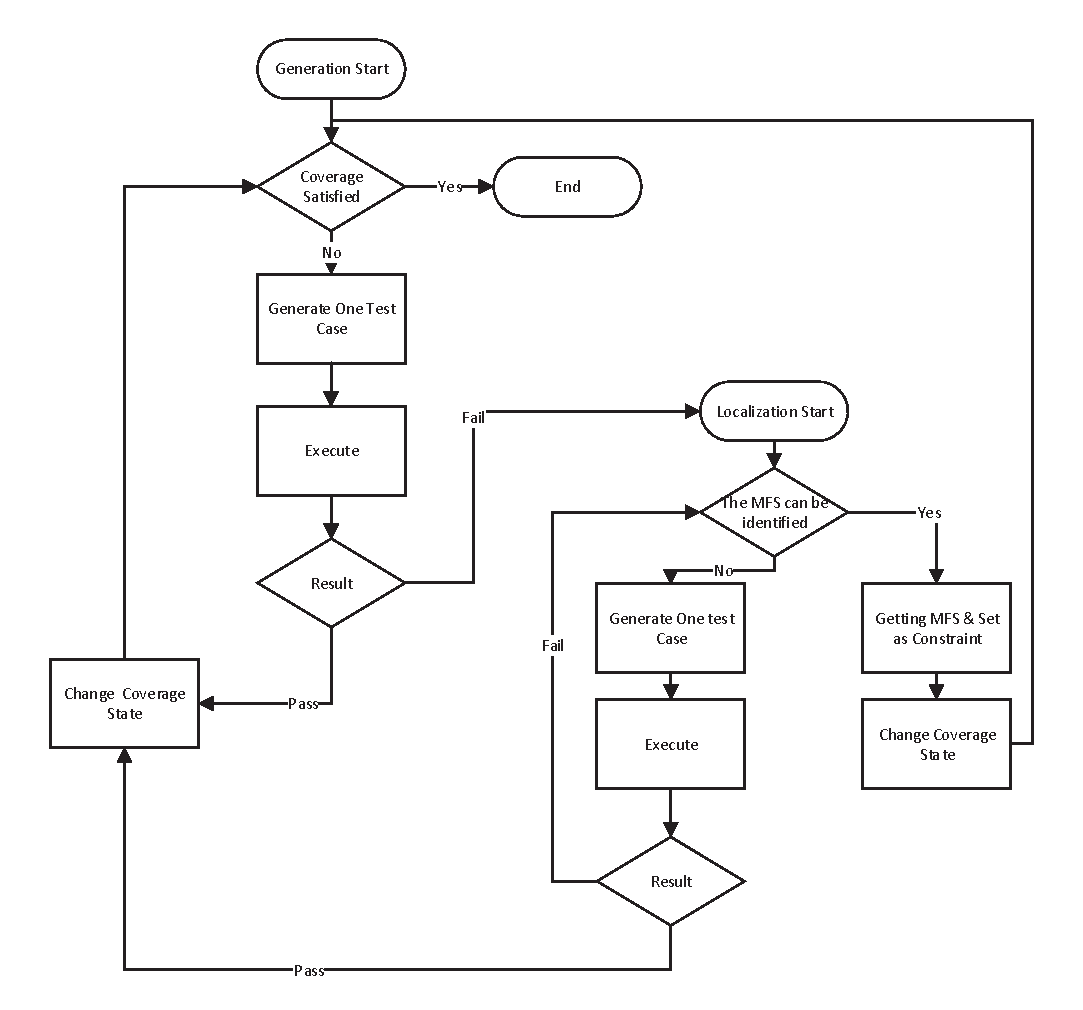
\includegraphics[width=3.4in]{baicOutline.eps}
\caption{New Framework of CT}
\label{new-life}
\end{figure}

In specific, this new framework works as follows: First, it will check whether all the needed schemas is covered or not. Commonly the target of CT is to cover all the $t$-valued schemas, with $t$ normally be assigned to be 2 or 3. Then if the coverage currently is not satisfied, it will generate a new test case to cover the schemas that is still not be covered as more as possible. After that, it will execute this test case with the outcome of the execution either be pass (executed normally, i.e., doesn't triggered an exception, violate the expected oracle or the like) or fail (on the contrary). When the test case pass the execution, we will recompute the coverage state, as all the schemas in the passing test case are regarded as error-irrelevant. As a result, the schemas that wasn't covered before will be determined to be covered if it is contained in this newly generated test case. Otherwise if the test case fails, then we will start the MFS identify module, to isolate the MFS in this failing test case. One point that needs to be noted is that if the test case fails, we will not change the coverage state, as we can not figure out which schemas are responsible to this failure among all the schemas in this test case until we isolate them.

The identify module works almost the same way as traditional independent MFS identify process, i.e., repeats generating and executing additional test cases until it can get enough information to diagnose the MFS in the original failing test case. The only difference from traditional MFS identifying process is that we augment it by counting the coverage this module have contributed to the overall coverage. In detail, when the additional test case passes, we will label the schemas in these test cases as covered if it had not been covered before. And when the MFS is found at the end of this module, we will first set them as forbidden schemas that latter generated test cases should not contain them (Otherwise the test case must fail and it cannot contribute to more coverage), second all the $t$-value schemas that are \emph{related} to these MFS will be set as covered. Here the \emph{related} indicates the following three types of $t$-value schemas:

First, the MFS \textbf{themselves}. Note that we haven't change the coverage state after the generated test case fails (both for the generation and identify module ), so these MFS will never be covered as they always appear in these failing test cases.

Second, the schemas that are the \textbf{parent-schemas} of these MFS. By definition of the parent-schemas (Definition 3), we can find if the test case contain the parent-schemas, it must also contain all its sub-schemas. So every test case contain the parent-schemas of the MFS must fail after execution. As a result, they will never be covered as we don't change coverage state for failing test cases.

Third, those \textbf{implicit forbidden} schemas, which was first introduced in \cite{cohen2007interaction}.  This type of schemas are caused by the conjunction of multiple MFS. For example, for a SUT with three parameters, and each parameter has two values, i.e., SUT(2, 2, 2). If there are two MFS for this SUT, which are (1, -, 1) and (0, 1, -). Then the schema (-, 1, 1) is the implicit forbidden schema. This is because for any test case that contain this schema, it must contain either (1, -, 1) or (0, 1, -). As a result, (-, 1, 1) will never be covered as all the test cases contain this schema will fail and so that we will not change the coverage state. In fact, by Definition 4, they can be deemed as faulty combinations.

As we all know, the terminating condition of the CT framework is to cover all the $t$-value schemas. Then since the three types of schemas will never be covered in our new CT framework, we must force to set them as covered after the execution of the identify module, so that the overall process can stop.

%This is because this MFS will be forbidden to appear in the following generated test cases, so its parent-schemas and itself will never be covered next. And if some of them are $t$-value schemas, then the generation process will never stop as these schemas will never be covered. So to avoid this, we force to label them to be covered in prior.
% based on the outcomes of these additional test cases; The only difference is that
%
%we just augment this module with counting the coverage this module have contributed to the overall coverage. In detail, we will count the uncovered schemas in the passing additional test cases as previously generated passing test cases. We still don't count the schemas in these failing additional test cases, instead, we will handle these identified MFS
%  Another important connection is that when we find the MFS in the failing test cases, there are two work needed to be completed: 1) we should make them as the constraint, such that the latter generated test cases should not contained this MFS. 2) the coverage this MFS and the schemas that related to this MFS should also set to be covered, as since we should not contain the MFS, then these schemas will not be covered. Then to make the overall generation process stop, we need to set them as "covered".


More details of these two important parts are as follows:

1) \emph{Generation} :
We adopt the one-test-case-one-time method as the basic skeleton of the generation process. And as discussed in section 3.1, we should account for the MFS to let them not appear in the latter generated test cases, which should be handled as the constraints--forbidden tuples. Our test case generation with consideration for constraints is inspired by the Cohen's AETG-SAT, based on which we give an more general approach that can be applied on more one-test-one-time generation methods.  The detail of how to generate one test case is described in Algorithm 1.

\begin{algorithm}
  \caption{Generate One test Case}
  \begin{algorithmic}[1]
     \Require
     $Param$ \Comment{values set that each option can take}

     $S_{MFS}$ \Comment{the set of MFS that currently isolated}

     $T_{uncovered}$ \Comment{the schemas that are still uncovered}
     %$s_{fixed}$ \Comment{fixed part}

     \Ensure  $test$ \Comment{the generate test case}

    % \While{\textbf{not} $t_{uncovered}$ is not empty}
      \State $Candidate_{test} \leftarrow empty Set$
      \While{$Candidate_{test}.size$ is not satisfied}
       \State $test \leftarrow emptyArray(Param.size)$
       \ForAll {$factor \in test$}
           \State   $value \leftarrow select(T_{uncovered},Param,factor)$
            \While{\textbf{not} $CheckCS(value, S_{MFS})$}
              \State $value \leftarrow repick(T_{uncovered},Param,factor) $
           \EndWhile
           \State $test.set(factor, value)$
       \EndFor
        \State $Candidate_{test}.append(test)$
       \EndWhile
       \State $best \leftarrow select(Candidate_{test})$
%       \State $t_{new} \leftarrow s_{fixed} \bigcup s_{mutant} $
%       \State $result \leftarrow execute(t_{new})$
%       \If {$result == PASS\ or\ result ==  F_{m}$}
%         \State \Return $t_{new}$
%       \Else
%         \State continue
%       \EndIf
 %   \EndWhile

     \State \Return $best$
  \end{algorithmic}
\end{algorithm}

This algorithm first gives a candidate set which initially is set to be empty (line 1). We lastly will fill up the set and select a best test case according to some criteria (line 13). For greedy algorithms like AETG \cite{cohen1997aetg} this criteria may be the test case which contain the most uncovered schemas.  A candidate test case in this set is constructed by assigning specific values to each parameter in this test case. It is noted that we didn't specify that in which order these factors should be assigned, as this varies with different One-test-one-time generation methods. For each parameter under assignment (line 4), the value that is selected must satisfy two requirements: first, it should ensure that the test case under construction could cover as many uncovered schemas as possible (line 5); second, it must ensure that the test case under construction should \textbf{not} contain any MFS (line 6 - 8).


The first requirement is usually fulfilled by some heuristic selection, e.g., to choose the value for the parameter that is contained in the most uncovered schemas \cite{cohen1997aetg}. To fulfill the second requirement, a constraint satisfaction modeling is needed. A general model is as following:

\begin{alignat}{2}
& X = { P_{1}, P_{2}, P_{3}, P_{n} } \\
& D = { D_{1}, D_{2}, ... D_{n} } \\
& C = {C_{assignment}, C_{MFS}}
%\end{aligned}
\end{alignat}

In this formula, $X$ is the parameters in the SUT and $D$ is a set of the respective domains of values that each each parameter can take. $C$ is the set of constraints. Then this model evaluates that whether a test case can be found, i.e., each parameter $P_{i}$ takes a specific value  $D_{i}$, so that it will not violate any constraint in $C$. For the constraints in $C$, $C_{assignment}$ indicates these parameters that have been assigned values. For example, if we have assigned parameter $P_{i}$ with value $d_{i}$, and $P_{j}$ with $d_{j}$, then this constraint will be formulated as $(P_{i} = d_{i}\ \&\&\ P_{j} == d_{j})$. $C_{MFS}$ modeled those identified MFS will be modeled as forbidden tuples of parameter values. For example, if (- 1 - 0) is the MFS, it will be transformed as forbidden rule $\urcorner ( P_{2} = 1\ \&\&\ P_{4} == 0)$.

So when using this model, we can check whether a value should be assigned to the current parameter(line 6) by putting it into the $C_{assignment}$. Note that the constraints checking part of our algorithm does not aim to optimising for the performance like running-time, iteration number or the like. Some study \cite{cohen2008constructing}, by exploiting the SAT history or setting the threshold, can significantly improve such performance. In this paper, however, we will not discuss the details for those techniques. Instead, we want to make the overall generation process more general and fit for the framework listed in Figure \ref{new-life}.

%However, our algorithm is powerful enough and properly adaptively to the framework we proposed.
% as we think to ,  is the most ada way for . We adopt the Need constraint.  Inspired by the Constraint AETG work by Cohen, we .

2) \emph{Isolation} : %ֻѡfixed��Ȼ���������ƣ�Ȼ���ص�˵��һ��fixed
The isolation process should also be adjusted to adapt to the new CT framework. From Figure \ref{new-life}, we can find some part of this process to isolate the MFS is similar to that of the $generation$ module, i.e., they all need to repeat generating test cases until reach some criteria. As for the additional test cases generated in the isolation process, we should also take care that it should not contain the previously isolated MFS. To achieve this goal, the constraints checking process is also needed like Algorithm 1. Another point that needs to be noted is that the additional test cases generated in the isolation process can also contribute the coverage. As the overall testing process aims to cover all the $t$-value schemas, so if those additional test cases can cover more uncovered $t$-value schemas, the overall testing process can stop earlier.  As a result, the overall test cases generated can be reduced. Based on the two points, the additional test cases generation in the CT isolation should be refined as in Algorithm 2.
\begin{algorithm}
  \caption{Test Case generation in isolation process}
  \begin{algorithmic}[1]
     \Require

     $f_{original}$ \Comment{original failing test case}
  %   $S_{isolated}$ \Comment{currently identified MFS}


     $S_{MFS}$ \Comment{previously identified MFS}

     $s_{fixed}$ \Comment{fixed part that should not be changed}

     $T_{uncovered}$ \Comment{the schemas that are still uncovered}

    $Param$ \Comment{values set that each option can take}


%     \Ensure  $t_{new}$ \Comment{the regenerate test case}

     \Ensure  $t_{new}$ \Comment{the regenerate test case}

     \State $Candidate_{test} \leftarrow empty Set$

      \While{$Candidate_{test}.size$ is not satisfied}
       \State $test \leftarrow emptyArray(Param.size)$
           \State $s_{mutant} \leftarrow f_{original} - s_{fixed}$
       \ForAll {$factor \in s_{mutant}$}
           \State   $value \leftarrow select(T_{uncovered},Param,factor)$
       %    \While{}
%           \EndWile{}
       %   \State $opt \leftarrow opt' \ s.t.\ opt' \in Param[i]\ and\ opt' != opt$
          \While{ \textbf{not} CheckCS(value, $S_{MFS}$) || value ==  GetValue(factor, $f_{original}) $}
            \State  $value \leftarrow repick(T_{uncovered},Param,factor)$
          \EndWhile
       \EndFor

%       \ForAll {$factor \in test$}
%           \State   $value \leftarrow select(T_{uncovered},Param,opt)$
%            \While{\textbf{not} $CheckSat(test, S_{MFS})$}
%              \State $value \leftarrow repick(T_{uncovered},Param,opt) $
%           \EndWhile
%           \State $test.set(factor, value)$
%       \EndFor
        \State $Candidate_{test}.append(test)$
       \EndWhile
       \State $best \leftarrow select(Candidate_{test})$

 %    \While{\textbf{not} MeetEndCriteria()}
%       \State $s_{mutant} \leftarrow f_{original} - s_{fixed}$
%       \ForAll {$opt \in s_{mutant}$}
%          \State $i = getIndex(Param,opt) $
%          \State $opt \leftarrow opt' \ s.t.\ opt' \in Param[i]\ and\ opt' != opt$
%          \While{ \textbf{not} CheckSat(test, $S_{MFS}$)}
%            \State $opt \leftarrow opt' \ s.t.\ opt' \in Param[i]\ and\ opt' != opt$
%          \EndWhile
%       \EndFor
%       \State $t_{new} \leftarrow s_{fixed} \bigcup s_{mutant} $
%       \State $result \leftarrow execute(t_{new})$
%       \If {$result == PASS\ or\ result ==  F_{m}$}
%         \State \Return $t_{new}$
%       \Else
%         \State continue
%       \EndIf
%     \EndWhile

     \State \Return \emph{best}
    % \While{\textbf{not} FindMFS()}
%       \State $s_{mutant} \leftarrow t_{original} - s_{fixed}$
%       \State $test \leftarrow initial(s_{fixed})$
%       \ForAll {$opt \in s_{mutant}$}
%          \State $i = getIndex(Param,opt) $
%          \State $opt \leftarrow opt' \ s.t.\ opt' \in Param[i]\ and\ opt' != opt$
%          \While{\textbf{not} $CheckSat(test, S_{MFS})$}
%              \State $value \leftarrow repick(Param,i) $
%           \EndWhile
%           \State $test.set(factor, value)$
%       \EndFor
%       \State $t_{new} \leftarrow s_{fixed} \bigcup s_{mutant} $
%       \State $result \leftarrow execute(t_{new})$
%       \If {$result == PASS$}
%         \State  $Update(t_{uncovered})$
%       \Else
%         \State continue
%       \EndIf
%     \EndWhile
%
%     \State $S_{MFS}.append(newMFS)$.
%     \State $t_{newCovered} \leftarrow FindingTschemas(S_{MFS})$
%     \State $t_{uncovered}.reduce(t_{newCovered})$
  \end{algorithmic}
\end{algorithm}

We can observe that this algorithm is very similar to Algorithm 1. This can be easily understood, as the the target of Algorithm 2 is also the approach that can make the isolation to generate more uncovered tuples as well as to not contain the previous isolated MFS. Two different parts are:

This is mainly based on the fact that the machinaim of MFS isoaltion is \emph{comparing}, that is, to compare the different schemas between the passing and failing test cases. And the fixed part is refer to the common part that is validated to error-irrelevant or not.


After the MFS are identified, some related schemas should be set as covered, i.e., these three types of schemas as we discussed before. The algorithm that seeks to handling these three types of schemas is listed in Algorithm 3.

%For example, consider the system has three parameters, and each parameter has two values that can be assigned, when we find the (0 1 -) and (1 - 0) are the MFS for this system, the schema (- 1 0) should also not appear, as when we generate test case that contain (- 1 0), i.e., either it contain MFS (0 1 -) for test case (0 1 0) or contain the MFS (1 - 0) for test case (1 1 0). And if we find the lower degree MFS like (0 - -), the forbidden schemas will be even more, as all the two-degree schemas contain this 1-degree schema should set to be covered. This problem is called the implicit constraints, firstly proposed by Cohen.

%So we just to find the different, that is, when finding is still the same as before: 1) the additional test case should not contain the MFS, if cannot find, set the test as . 2) when update the MFS set. and coverage set.

\begin{algorithm}
  \caption{Changing coverage after identification of MFS}
  \begin{algorithmic}[1]
     \Require

    % $t_{original}$ \Comment{original failing test case}
     $S_{isolated}$ \Comment{currently identified MFS}


     $S_{MFS}$ \Comment{previously identified MFS}

     $T_{uncovered}$ \Comment{the schemas that are still uncovered}

   %  $Param$ \Comment{values set that each option can take}


%     \Ensure  $t_{new}$ \Comment{the regenerate test case}
     \ForAll  {$s \in S_{isolated}$}
       \State $S_{MFS}.append(s)$
     \EndFor


     \ForAll {$s  \in  S_{isolated}$}
       \If {$s$\ is\ $t$-degree\ schema}
          \State $T_{uncovered}.remove(s)$
       \EndIf
       \ForAll {$s_{p}$\ is\ parent-schema\ of\ $s$}
         \If {$s_{p}$\ is\ $t$-degree\ schema}
          \State $T_{uncovered}.remove(s_{p})$
         \EndIf
       \EndFor
     \EndFor
%           % \State $S_{MFS}.append(s)$
%     \EndFor
%     \ForAll {$s$ \in S_{isolated}}
%       \If {$s$\ is\ $t$-degree\ schema}
%          \State set $s$ covered
%       \Endif
           % \State $S_{MFS}.append(s)$
%     \EndFor
     \ForAll {$t \in T_{uncovered}$}
       \If {\textbf{not} $CheckCS(t, S_{MFS})$}
         \State  $T_{uncovered}.remove(t)$
       \EndIf
     \EndFor
  \end{algorithmic}
\end{algorithm}

 In this algorithm, we firstly append the newly isolated MFS into the global MFS set (line 1 - 3), so that we can use them in the following generation and isolation processes. Then for each newly isolated MFS, we will set them as covered, i.e., remove them from the uncovered set, if they are $t$-degree schemas (line 4 - 7). This is the first type of schemas --\emph{themselves}. For each $t$-degree parent-schema of these newly isolated MFS, we will also remove them from the uncovered set (line 8 - 12), as they are the second type of schemas --  \emph{parent-schemas}. The last type, i.e., \emph{implicit forbidden schemas}, is the toughest one. To remove them, we need to search through each potential schema in the uncovered schemas set (line 14), and judge if it is the implicit forbidden schema (line 16) by sat checking. This checking process is the same as we discussed in the generation and isolation process.

% To find them from the uncovered set, we use a sat solver to
%he uncovetred  search through the uncovered schemas set (line 4), to eliminate these schemas that cannot avoid some MFS when extend these schemas into a test case(line 5 - 7).

%3) Setting constraint, and change coverage.



%Then the generation should not include, the characterization is should.

%To implement such framework, the most important is to share the information. In specific, to, we use the SAT solver. And when , we should change the coverage information. Our detail implementation for this framework is list in Algorithm.

With this newly framework, when we re-consider the example in Table \ref{tradition-gi} in section 3.1,  we can get the following result listed in Table \ref{new-gi}.
\begin{table}[h]
\caption{newly generation-isolation life-circle}
\label{new-gi}
\center
\begin{tabular}{llllll|llllll}
 & \multicolumn{4}{c}{\bfseries generation}& & \multicolumn{6}{c}{\bfseries isolation} \\
%\multicolumn{5}{c}{\bfseries test case} & \bfseries Outcome \\
$t_{1}$* & \multicolumn{4}{l}{0 \ \ \ \ 0 \ \ \ \  0  \ \ \ \  0 } & Fail & \multicolumn{6}{l}{}\\
\multicolumn{5}{l}{}& & $t_{2}$* &\multicolumn{4}{l}{1  \ \ \ \  0 \ \ \ \  0 }& Pass \\
\multicolumn{5}{l}{}& &$t_{3}$* &\multicolumn{4}{l}{0  \ \ \ \  1 \ \ \ \  0 } & Fail \\
\multicolumn{5}{l}{}& &$t_{4}$* &\multicolumn{4}{l}{0  \ \ \ \  0 \ \ \ \  1 } & Fail \\
\multicolumn{5}{l}{}& &\multicolumn{6}{l}{ \bfseries{MFS}: $(0, - , -)$ }  \\
$t_{5}$* &\multicolumn{4}{l}{1  \ \ \ \  1 \ \ \ \  1 } & Pass & \multicolumn{6}{l}{}\\
$t_{6}$* &\multicolumn{4}{l}{1  \ \ \ \  0 \ \ \ \  1 } & Pass & \multicolumn{6}{l}{}\\
$t_{7}$* &\multicolumn{4}{l}{1  \ \ \ \  1 \ \ \ \  0 } & Pass & \multicolumn{6}{l}{}\\
\end{tabular}
\end{table}

This table consists of two main columns, where the left indicates the generation part while the right column indicates the isolation process.

Up to now, all the 2-degree schemas are covered, in detail, (1  1 -) (1 - 1) (- 1 1) are covered by passing test case (1 1 1), (1 0 -) (1 - 0) (- 0 0) are covered by passing test case (1 0 0), (- 0 1) and (- 1 0) are covered by test case (1 0 1) and (1 1 0) respectively. Those schemas related to (0 - -) such as (0 - 1), (0 0 -) will not be covered as the (0 - -) is the MFS.  All the generated 7 test cases are not duplicated with each other (all marked *), we can find the overall generated test case are one less than the traditional approaches in Table \ref{tradition-gi}. Another advances of our approach is that our approach provide a stronger covering criteria than traditional covering array.

%\subsection{Description}
%
%
%\subsection{A case study}

\section{empirical studies}

\subsection{Compare with Traditional First-Gen-Latter-Identify}

\subsubsection{Study setup}

\subsubsection{Result and discussion}

\subsection{Compare with the FDA-CIT}

\subsubsection{Study setup}


\subsubsection{Result and discussion}


\subsection{Comparing with Error locating Array}
Erray locating array \cite{colbourn2008locating,martinez2009locating} is a well-designed set of test cases, such that it can support not only failure detection, but also the identification for the MFS of the failure.

\subsubsection{Study setup}


%Additionally, comparisons between the augmented approaches and three traditional ones will be quantified.

\subsubsection{Result and discussion}


\subsection{Threats to validity}


\section{related works}


\section{Conclusions}


%\end{document}  % This is where a 'short' article might terminate

%ACKNOWLEDGMENTS are optional
%\section{Acknowledgments}
%This section is optional; it is a location for you
%to acknowledge grants, funding, editing assistance and
%what have you.  In the present case, for example, the
%authors would like to thank Gerald Murray of ACM for
%his help in codifying this \textit{Author's Guide}
%and the \textbf{.cls} and \textbf{.tex} files that it describes.

%
% The following two commands are all you need in the
% initial runs of your .tex file to
% produce the bibliography for the citations in your paper.
\bibliographystyle{abbrv}
%\bibliographystyle{unsrt}
\bibliography{sigproc}  % sigproc.bib is the name of the Bibliography in this case
% You must have a proper ".bib" file
%  and remember to run:
% latex bibtex latex latex
% to resolve all references
%
% ACM needs 'a single self-contained file'!
%
%APPENDICES are optional
%\balancecolumns
%\appendix
%%Appendix A
\end{document}
